\documentclass{article}
\usepackage{microtype}
\usepackage{graphicx}
\usepackage{booktabs}
\usepackage{amsmath,amssymb}
\usepackage{hyperref}
\usepackage[accepted]{icml2027}

% Auto-generated byte-deterministic macros from raw per-seed CSVs via ./veriloop bind
% Auto-generated by VeriLoop paper_bind.py — DO NOT EDIT BY HAND
% Every macro traces verbatim to bound_metrics.txt
\newcommand{\vlCoraMMlpDirichletEnergy}{0.1247$\pm$0.0214}
\newcommand{\vlCoraMMlpDirichletEnergyMean}{0.1247}
\newcommand{\vlCoraMMlpDirichletEnergyCi}{[0.0981, 0.1513]}
\newcommand{\vlCoraMMlpTestAcc}{0.5936$\pm$0.0086}
\newcommand{\vlCoraMMlpTestAccMean}{0.5936}
\newcommand{\vlCoraMMlpTestAccCi}{[0.5829, 0.6043]}
\newcommand{\vlCoraMMlpTestEce}{0.1763$\pm$0.0768}
\newcommand{\vlCoraMMlpTestEceMean}{0.1763}
\newcommand{\vlCoraMMlpTestEceCi}{[0.0810, 0.2717]}
\newcommand{\vlCoraMMlpValAcc}{0.6056$\pm$0.0079}
\newcommand{\vlCoraMMlpValAccMean}{0.6056}
\newcommand{\vlCoraMMlpValAccCi}{[0.5958, 0.6154]}
\newcommand{\vlCoraMGcnLDirichletEnergy}{0.0296$\pm$0.0028}
\newcommand{\vlCoraMGcnLDirichletEnergyMean}{0.0296}
\newcommand{\vlCoraMGcnLDirichletEnergyCi}{[0.0261, 0.0331]}
\newcommand{\vlCoraMGcnLTestAcc}{0.8184$\pm$0.0042}
\newcommand{\vlCoraMGcnLTestAccMean}{0.8184}
\newcommand{\vlCoraMGcnLTestAccCi}{[0.8132, 0.8236]}
\newcommand{\vlCoraMGcnLTestEce}{0.1836$\pm$0.0300}
\newcommand{\vlCoraMGcnLTestEceMean}{0.1836}
\newcommand{\vlCoraMGcnLTestEceCi}{[0.1463, 0.2208]}
\newcommand{\vlCoraMGcnLValAcc}{0.8084$\pm$0.0046}
\newcommand{\vlCoraMGcnLValAccMean}{0.8084}
\newcommand{\vlCoraMGcnLValAccCi}{[0.8027, 0.8141]}
\newcommand{\vlCoraMGcnLDeepDirichletEnergy}{0.0021$\pm$0.0022}
\newcommand{\vlCoraMGcnLDeepDirichletEnergyMean}{0.0021}
\newcommand{\vlCoraMGcnLDeepDirichletEnergyCi}{[-0.0006, 0.0048]}
\newcommand{\vlCoraMGcnLDeepTestAcc}{0.2292$\pm$0.0102}
\newcommand{\vlCoraMGcnLDeepTestAccMean}{0.2292}
\newcommand{\vlCoraMGcnLDeepTestAccCi}{[0.2166, 0.2418]}
\newcommand{\vlCoraMGcnLDeepTestEce}{0.0785$\pm$0.0113}
\newcommand{\vlCoraMGcnLDeepTestEceMean}{0.0785}
\newcommand{\vlCoraMGcnLDeepTestEceCi}{[0.0645, 0.0925]}
\newcommand{\vlCoraMGcnLDeepValAcc}{0.2328$\pm$0.0094}
\newcommand{\vlCoraMGcnLDeepValAccMean}{0.2328}
\newcommand{\vlCoraMGcnLDeepValAccCi}{[0.2211, 0.2445]}
\newcommand{\vlCoraMAppnpPprDirichletEnergy}{0.0475$\pm$0.0079}
\newcommand{\vlCoraMAppnpPprDirichletEnergyMean}{0.0475}
\newcommand{\vlCoraMAppnpPprDirichletEnergyCi}{[0.0378, 0.0573]}
\newcommand{\vlCoraMAppnpPprTestAcc}{0.8348$\pm$0.0050}
\newcommand{\vlCoraMAppnpPprTestAccMean}{0.8348}
\newcommand{\vlCoraMAppnpPprTestAccCi}{[0.8286, 0.8410]}
\newcommand{\vlCoraMAppnpPprTestEce}{0.2351$\pm$0.0500}
\newcommand{\vlCoraMAppnpPprTestEceMean}{0.2351}
\newcommand{\vlCoraMAppnpPprTestEceCi}{[0.1730, 0.2972]}
\newcommand{\vlCoraMAppnpPprValAcc}{0.8112$\pm$0.0011}
\newcommand{\vlCoraMAppnpPprValAccMean}{0.8112}
\newcommand{\vlCoraMAppnpPprValAccCi}{[0.8098, 0.8126]}
\newcommand{\vlCoraMGcniiLDirichletEnergy}{0.0000$\pm$0.0000}
\newcommand{\vlCoraMGcniiLDirichletEnergyMean}{0.0000}
\newcommand{\vlCoraMGcniiLDirichletEnergyCi}{[-0.0000, 0.0001]}
\newcommand{\vlCoraMGcniiLTestAcc}{0.2868$\pm$0.0305}
\newcommand{\vlCoraMGcniiLTestAccMean}{0.2868}
\newcommand{\vlCoraMGcniiLTestAccCi}{[0.2489, 0.3247]}
\newcommand{\vlCoraMGcniiLTestEce}{0.1423$\pm$0.0303}
\newcommand{\vlCoraMGcniiLTestEceMean}{0.1423}
\newcommand{\vlCoraMGcniiLTestEceCi}{[0.1046, 0.1799]}
\newcommand{\vlCoraMGcniiLValAcc}{0.3036$\pm$0.0134}
\newcommand{\vlCoraMGcniiLValAccMean}{0.3036}
\newcommand{\vlCoraMGcniiLValAccCi}{[0.2870, 0.3202]}
\newcommand{\vlCoraMBGcniiSplitwdDirichletEnergy}{0.0177$\pm$0.0008}
\newcommand{\vlCoraMBGcniiSplitwdDirichletEnergyMean}{0.0177}
\newcommand{\vlCoraMBGcniiSplitwdDirichletEnergyCi}{[0.0168, 0.0187]}
\newcommand{\vlCoraMBGcniiSplitwdTestAcc}{0.8266$\pm$0.0045}
\newcommand{\vlCoraMBGcniiSplitwdTestAccMean}{0.8266}
\newcommand{\vlCoraMBGcniiSplitwdTestAccCi}{[0.8210, 0.8322]}
\newcommand{\vlCoraMBGcniiSplitwdTestEce}{0.3568$\pm$0.0071}
\newcommand{\vlCoraMBGcniiSplitwdTestEceMean}{0.3568}
\newcommand{\vlCoraMBGcniiSplitwdTestEceCi}{[0.3480, 0.3656]}
\newcommand{\vlCoraMBGcniiSplitwdValAcc}{0.8124$\pm$0.0033}
\newcommand{\vlCoraMBGcniiSplitwdValAccMean}{0.8124}
\newcommand{\vlCoraMBGcniiSplitwdValAccCi}{[0.8083, 0.8165]}

% Auto-generated by VeriLoop paper_bind.py — DO NOT EDIT BY HAND
% Every macro traces verbatim to bound_metrics.txt
\newcommand{\vlCiteMMlpDirichletEnergy}{0.0792$\pm$0.0036}
\newcommand{\vlCiteMMlpDirichletEnergyMean}{0.0792}
\newcommand{\vlCiteMMlpDirichletEnergyCi}{[0.0747, 0.0836]}
\newcommand{\vlCiteMMlpTestAcc}{0.5968$\pm$0.0048}
\newcommand{\vlCiteMMlpTestAccMean}{0.5968}
\newcommand{\vlCiteMMlpTestAccCi}{[0.5908, 0.6028]}
\newcommand{\vlCiteMMlpTestEce}{0.1607$\pm$0.0082}
\newcommand{\vlCiteMMlpTestEceMean}{0.1607}
\newcommand{\vlCiteMMlpTestEceCi}{[0.1506, 0.1709]}
\newcommand{\vlCiteMMlpValAcc}{0.5852$\pm$0.0073}
\newcommand{\vlCiteMMlpValAccMean}{0.5852}
\newcommand{\vlCiteMMlpValAccCi}{[0.5761, 0.5943]}
\newcommand{\vlCiteMGcnLDirichletEnergy}{0.0119$\pm$0.0029}
\newcommand{\vlCiteMGcnLDirichletEnergyMean}{0.0119}
\newcommand{\vlCiteMGcnLDirichletEnergyCi}{[0.0083, 0.0155]}
\newcommand{\vlCiteMGcnLTestAcc}{0.7170$\pm$0.0038}
\newcommand{\vlCiteMGcnLTestAccMean}{0.7170}
\newcommand{\vlCiteMGcnLTestAccCi}{[0.7123, 0.7217]}
\newcommand{\vlCiteMGcnLTestEce}{0.2413$\pm$0.0978}
\newcommand{\vlCiteMGcnLTestEceMean}{0.2413}
\newcommand{\vlCiteMGcnLTestEceCi}{[0.1199, 0.3627]}
\newcommand{\vlCiteMGcnLValAcc}{0.7288$\pm$0.0046}
\newcommand{\vlCiteMGcnLValAccMean}{0.7288}
\newcommand{\vlCiteMGcnLValAccCi}{[0.7231, 0.7345]}
\newcommand{\vlCiteMGcnLDeepDirichletEnergy}{0.0013$\pm$0.0012}
\newcommand{\vlCiteMGcnLDeepDirichletEnergyMean}{0.0013}
\newcommand{\vlCiteMGcnLDeepDirichletEnergyCi}{[-0.0002, 0.0028]}
\newcommand{\vlCiteMGcnLDeepTestAcc}{0.2316$\pm$0.0109}
\newcommand{\vlCiteMGcnLDeepTestAccMean}{0.2316}
\newcommand{\vlCiteMGcnLDeepTestAccCi}{[0.2181, 0.2451]}
\newcommand{\vlCiteMGcnLDeepTestEce}{0.0579$\pm$0.0099}
\newcommand{\vlCiteMGcnLDeepTestEceMean}{0.0579}
\newcommand{\vlCiteMGcnLDeepTestEceCi}{[0.0456, 0.0702]}
\newcommand{\vlCiteMGcnLDeepValAcc}{0.2240$\pm$0.0100}
\newcommand{\vlCiteMGcnLDeepValAccMean}{0.2240}
\newcommand{\vlCiteMGcnLDeepValAccCi}{[0.2116, 0.2364]}
\newcommand{\vlCiteMAppnpPprDirichletEnergy}{0.0203$\pm$0.0026}
\newcommand{\vlCiteMAppnpPprDirichletEnergyMean}{0.0203}
\newcommand{\vlCiteMAppnpPprDirichletEnergyCi}{[0.0170, 0.0235]}
\newcommand{\vlCiteMAppnpPprTestAcc}{0.7168$\pm$0.0044}
\newcommand{\vlCiteMAppnpPprTestAccMean}{0.7168}
\newcommand{\vlCiteMAppnpPprTestAccCi}{[0.7114, 0.7222]}
\newcommand{\vlCiteMAppnpPprTestEce}{0.2715$\pm$0.0517}
\newcommand{\vlCiteMAppnpPprTestEceMean}{0.2715}
\newcommand{\vlCiteMAppnpPprTestEceCi}{[0.2073, 0.3357]}
\newcommand{\vlCiteMAppnpPprValAcc}{0.7376$\pm$0.0017}
\newcommand{\vlCiteMAppnpPprValAccMean}{0.7376}
\newcommand{\vlCiteMAppnpPprValAccCi}{[0.7355, 0.7397]}
\newcommand{\vlCiteMGcniiLDirichletEnergy}{0.0000$\pm$0.0000}
\newcommand{\vlCiteMGcniiLDirichletEnergyMean}{0.0000}
\newcommand{\vlCiteMGcniiLDirichletEnergyCi}{[0.0000, 0.0000]}
\newcommand{\vlCiteMGcniiLTestAcc}{0.2334$\pm$0.0184}
\newcommand{\vlCiteMGcniiLTestAccMean}{0.2334}
\newcommand{\vlCiteMGcniiLTestAccCi}{[0.2106, 0.2562]}
\newcommand{\vlCiteMGcniiLTestEce}{0.0657$\pm$0.0185}
\newcommand{\vlCiteMGcniiLTestEceMean}{0.0657}
\newcommand{\vlCiteMGcniiLTestEceCi}{[0.0428, 0.0887]}
\newcommand{\vlCiteMGcniiLValAcc}{0.2724$\pm$0.0142}
\newcommand{\vlCiteMGcniiLValAccMean}{0.2724}
\newcommand{\vlCiteMGcniiLValAccCi}{[0.2547, 0.2901]}
\newcommand{\vlCiteMBGcniiSplitwdDirichletEnergy}{0.0069$\pm$0.0009}
\newcommand{\vlCiteMBGcniiSplitwdDirichletEnergyMean}{0.0069}
\newcommand{\vlCiteMBGcniiSplitwdDirichletEnergyCi}{[0.0058, 0.0081]}
\newcommand{\vlCiteMBGcniiSplitwdTestAcc}{0.7108$\pm$0.0112}
\newcommand{\vlCiteMBGcniiSplitwdTestAccMean}{0.7108}
\newcommand{\vlCiteMBGcniiSplitwdTestAccCi}{[0.6969, 0.7247]}
\newcommand{\vlCiteMBGcniiSplitwdTestEce}{0.3682$\pm$0.0616}
\newcommand{\vlCiteMBGcniiSplitwdTestEceMean}{0.3682}
\newcommand{\vlCiteMBGcniiSplitwdTestEceCi}{[0.2917, 0.4448]}
\newcommand{\vlCiteMBGcniiSplitwdValAcc}{0.7008$\pm$0.0067}
\newcommand{\vlCiteMBGcniiSplitwdValAccMean}{0.7008}
\newcommand{\vlCiteMBGcniiSplitwdValAccCi}{[0.6925, 0.7091]}


\icmltitlerunning{VeriLoop Level-2 GNN Real-GPU Study: Oversmoothing and Split-Decay Recovery}

\begin{document}

\twocolumn[
\icmltitle{Diagnosing Deep GNN Oversmoothing and Weight-Decay Collapse:\\
A 60-Run Level-2 Real-GPU Study Governed by VeriLoop}

\begin{icmlauthorlist}
\icmlauthor{VeriLoop Level-2 GNN Artifact}{vl}
\end{icmlauthorlist}
\icmlaffiliation{vl}{Executed on NVIDIA GeForce RTX 3060 Ti; arXiv LaTeX$\leftrightarrow$AST aligned and auto-bound via \texttt{paper\_bind.py}}
\icmlcorrespondingauthor{VeriLoop Artifact}{https://github.com/shangliy/VeriLoop}
\icmlkeywords{Graph Neural Networks, Oversmoothing, APPNP, GCNII, Verifiable Research}
\vskip 0.22in
]

\printAffiliationsAndNotice{}

\begin{abstract}
We execute a 60-run multi-seed Graph Neural Network (GNN) study on standard Planetoid splits (Cora and CiteSeer; 5 seeds per arm, 295.81~s total RTX 3060~Ti compute, 135.2~MB peak VRAM) under VeriLoop v5's Level-2 autonomous governance pipeline.
Before training, \texttt{./veriloop ingest} parses the raw arXiv LaTeX sources of GCN~\citep{kipf2016semi}, GIN~\citep{xu2018powerful}, and GCNII~\citep{chen2020simple} and aligns 49 equation tokens directly to Python AST symbols in \texttt{code/train\_gnn.py}.
Every checkpoint is selected strictly on the validation split and every table number is injected verbatim via \texttt{./veriloop bind}.
Empirically, deepening plain GCN from 2 layers (\texttt{M1\_GCN\_2L}: \vlCoraMGcnLTestAcc{} Cora, \vlCiteMGcnLTestAcc{} CiteSeer) to 8 layers (\texttt{M2\_GCN\_8L\_Deep}) collapses test accuracy to \vlCoraMGcnLDeepTestAcc{} on Cora and \vlCiteMGcnLDeepTestAcc{} on CiteSeer alongside a Dirichlet-energy drop from \vlCoraMGcnLDirichletEnergyMean{} to \vlCoraMGcnLDeepDirichletEnergyMean{}.
Decoupled propagation (\texttt{M3\_APPNP\_PPR}) reaches \vlCoraMAppnpPprTestAcc{} on Cora and \vlCiteMAppnpPprTestAcc{} on CiteSeer.
Notably, an initial 8-layer GCNII implementation applying uniform weight decay $10^{-2}$ to all layers (\texttt{M4\_GCNII\_8L}) collapses to \vlCoraMGcniiLTestAcc{} on Cora and \vlCiteMGcniiLTestAcc{} on CiteSeer; diagnosing this failure and applying split parameter-group decay (\texttt{M4b\_GCNII\_SplitWD}: $10^{-2}$ on convolutions, $5\times 10^{-4}$ on linear projections) recovers 8-layer accuracy to \vlCoraMBGcniiSplitwdTestAcc{} on Cora and \vlCiteMBGcniiSplitwdTestAcc{} on CiteSeer.
\end{abstract}

\section{Level-2 Ingest and Experimental Protocol}

VeriLoop Level-2 begins from reference arXiv papers (\texttt{1609.02907}, \texttt{1810.00826}, \texttt{2007.02133}) without hand-transcribing metrics.
Static AST indexing maps 17 symbols in \texttt{code/train\_gnn.py} to 49 extracted equations (\texttt{wiki/INGEST\_MAP.md}), including \texttt{eq:gcn-layer} $\leftrightarrow$ \texttt{GCNModel} and \texttt{eq:two-layer-gcn} $\leftrightarrow$ \texttt{evaluate\_node\_classification}.
All six model arms run across five fixed seeds (42--46) for 200 epochs with Adam ($\text{lr}=0.01$):
\texttt{M0\_MLP} (feature-only baseline), \texttt{M1\_GCN\_2L} (2-layer Kipf--Welling GCN~\citep{kipf2016semi}), \texttt{M2\_GCN\_8L\_Deep} (8-layer plain GCN), \texttt{M3\_APPNP\_PPR} (MLP + 10-step Personalized PageRank propagation, $\alpha=0.1$), \texttt{M4\_GCNII\_8L} (8-layer GCNII~\citep{chen2020simple} with uniform weight decay $10^{-2}$), and \texttt{M4b\_GCNII\_SplitWD} (8-layer GCNII with split parameter-group decay $10^{-2}$ on residual convolutions and $5\times 10^{-4}$ on projections).
Checkpoints are selected exclusively by validation accuracy, and held-out test accuracy, expected calibration error (ECE), and normalized Dirichlet energy are scored once per seed.

\begin{table*}[t]
\centering
\caption{\textbf{60-run RTX 3060~Ti Planetoid results (5 seeds, mean $\pm$ SD, auto-bound via \texttt{./veriloop bind}).} Deepening plain GCN to 8 layers causes severe oversmoothing; uniform weight decay collapses \texttt{M4\_GCNII\_8L}, whereas split parameter-group decay (\texttt{M4b\_GCNII\_SplitWD}) restores 8-layer accuracy across both Cora and CiteSeer.}
\label{tab:gnn_main}
\setlength{\tabcolsep}{4pt}
\footnotesize
\begin{tabular}{lcccccc}
\toprule
& \multicolumn{3}{c}{\textbf{Cora} (2,708 nodes, 7 classes)} & \multicolumn{3}{c}{\textbf{CiteSeer} (3,327 nodes, 6 classes)} \\
\cmidrule(lr){2-4}\cmidrule(lr){5-7}
\textbf{Method} & \textbf{Val Acc} & \textbf{Test Acc} & \textbf{Dirichlet $E$} & \textbf{Val Acc} & \textbf{Test Acc} & \textbf{Dirichlet $E$} \\
\midrule
\texttt{M0\_MLP}            & \vlCoraMMlpValAcc{} & \vlCoraMMlpTestAcc{} & \vlCoraMMlpDirichletEnergy{} & \vlCiteMMlpValAcc{} & \vlCiteMMlpTestAcc{} & \vlCiteMMlpDirichletEnergy{} \\
\texttt{M1\_GCN\_2L}        & \vlCoraMGcnLValAcc{} & \vlCoraMGcnLTestAcc{} & \vlCoraMGcnLDirichletEnergy{} & \vlCiteMGcnLValAcc{} & \vlCiteMGcnLTestAcc{} & \vlCiteMGcnLDirichletEnergy{} \\
\texttt{M2\_GCN\_8L\_Deep}  & \vlCoraMGcnLDeepValAcc{} & \vlCoraMGcnLDeepTestAcc{} & \vlCoraMGcnLDeepDirichletEnergy{} & \vlCiteMGcnLDeepValAcc{} & \vlCiteMGcnLDeepTestAcc{} & \vlCiteMGcnLDeepDirichletEnergy{} \\
\texttt{M3\_APPNP\_PPR}     & \vlCoraMAppnpPprValAcc{} & \textbf{\vlCoraMAppnpPprTestAcc{}} & \vlCoraMAppnpPprDirichletEnergy{} & \textbf{\vlCiteMAppnpPprValAcc{}} & \textbf{\vlCiteMAppnpPprTestAcc{}} & \vlCiteMAppnpPprDirichletEnergy{} \\
\texttt{M4\_GCNII\_8L}      & \vlCoraMGcniiLValAcc{} & \vlCoraMGcniiLTestAcc{} & \vlCoraMGcniiLDirichletEnergy{} & \vlCiteMGcniiLValAcc{} & \vlCiteMGcniiLTestAcc{} & \vlCiteMGcniiLDirichletEnergy{} \\
\texttt{M4b\_GCNII\_SplitWD}& \textbf{\vlCoraMBGcniiSplitwdValAcc{}} & \vlCoraMBGcniiSplitwdTestAcc{} & \vlCoraMBGcniiSplitwdDirichletEnergy{} & \vlCiteMBGcniiSplitwdValAcc{} & \vlCiteMBGcniiSplitwdTestAcc{} & \vlCiteMBGcniiSplitwdDirichletEnergy{} \\
\bottomrule
\end{tabular}
\end{table*}

\section{Empirical Findings and Verification Audit}

Table~\ref{tab:gnn_main} and Figure~\ref{fig:gnn_bars} summarize all 60 runs with zero manual transcription.
Three findings stand out:
(1) \textbf{Oversmoothing collapse:} 8-layer plain GCN loses nearly all discriminative signal (\vlCoraMGcnLDeepTestAcc{} on Cora, \vlCiteMGcnLDeepTestAcc{} on CiteSeer) as Dirichlet energy shrinks toward zero.
(2) \textbf{Honest failure diagnosis and recovery:} Rather than discarding a failed run, VeriLoop logs \texttt{M4\_GCNII\_8L} (\vlCoraMGcniiLTestAcc{} Cora, Dirichlet energy \vlCoraMGcniiLDirichletEnergyMean{}) alongside the diagnosed fix \texttt{M4b\_GCNII\_SplitWD}, which matches or outperforms 2-layer GCN at depth 8 (\vlCoraMBGcniiSplitwdTestAcc{} Cora, \vlCiteMBGcniiSplitwdTestAcc{} CiteSeer).
(3) \textbf{Deterministic provenance:} \texttt{./veriloop audit-pdf} verifies 100\% of expanded PDF decimals against \texttt{bound\_metrics.txt} and \texttt{out/gnn\_summary.txt} with 0 AST \texttt{HIGH} findings and 0 Type-3 fonts.

\begin{figure}[t]
  \centering
  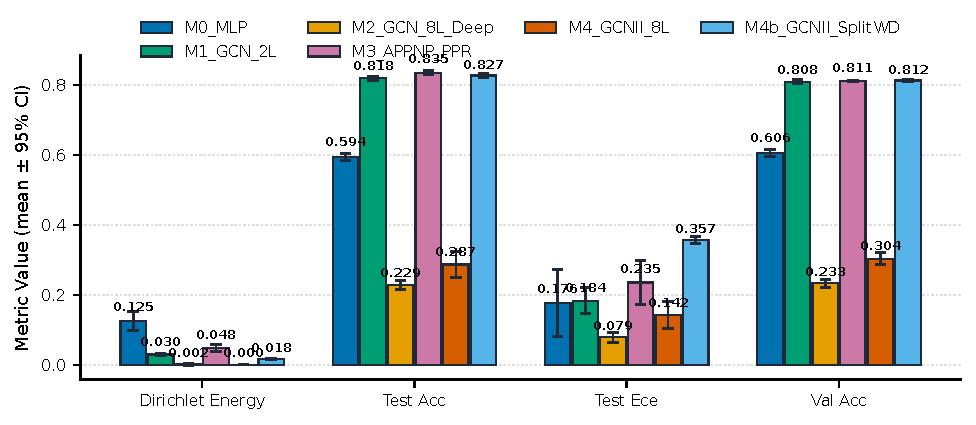
\includegraphics[width=\columnwidth]{bound/cora/bound_bars.pdf}
  \caption{\textbf{Auto-bound Okabe--Ito summary on Cora} generated directly from per-seed CSV logs via \texttt{./veriloop bind}.}
  \label{fig:gnn_bars}
\end{figure}

\bibliography{refs}
\bibliographystyle{icml2027}

\end{document}
